\section{Ejemplos de ejecución}
Se pueden encontrar encontrar multiples ejemplos de ejecución dentro del directorio \textit{ejemplos} en el repositorio. Veamos algunos:

Supongamos que tenemos 5 monedas:

\begin{lstlisting}
    [96, 594, 437, 674, 950]
\end{lstlisting}

Veamos lo que obtenemos al ejecutar en código el ejemplo que acabamos de ver:

\begin{center}
    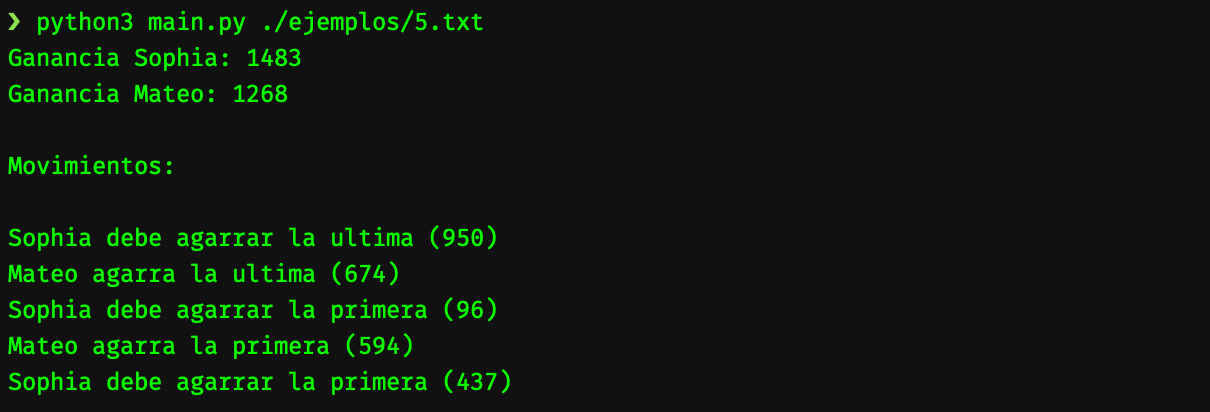
\includegraphics[scale = 0.6]{ {images/screen3.png} } 
\end{center}

Veamos la ejecución de otros ejemplos brindados por la cátedra:
\vskip0.5cm
Este ejemplo es con 10 monedas:
\begin{center}
    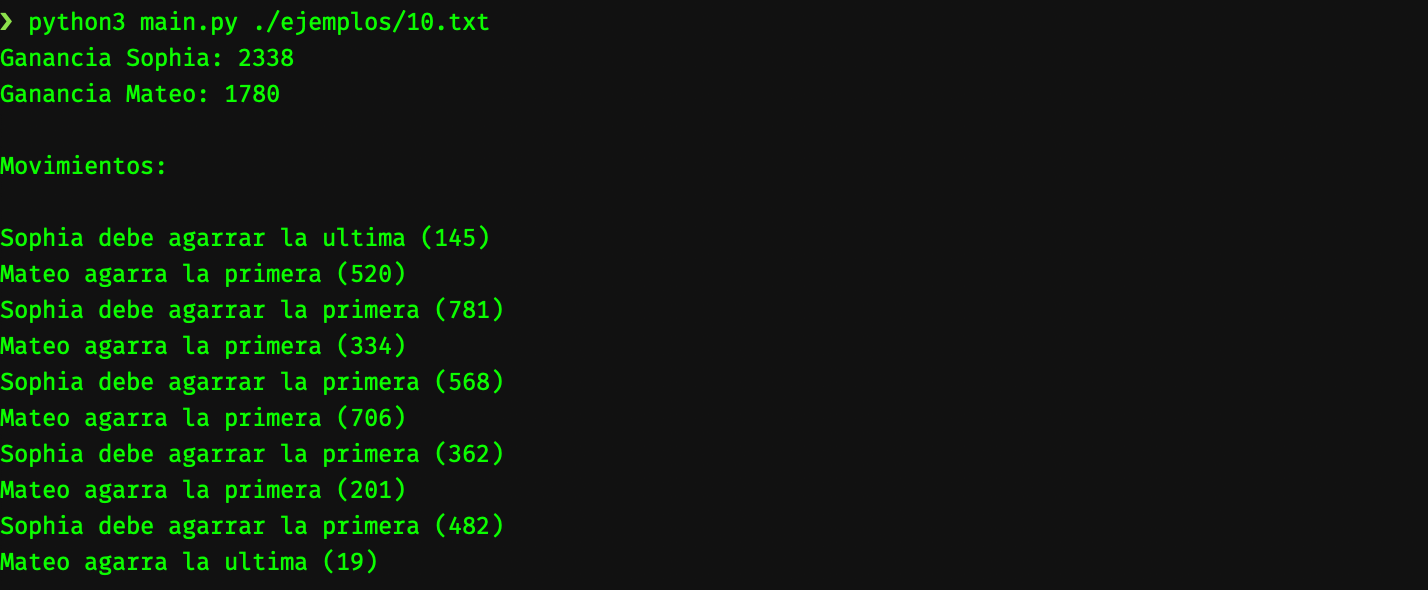
\includegraphics[scale = 0.6]{ {images/screen1.png} } 
\end{center}
Este ejemplo es con 25 monedas:
\begin{center}
    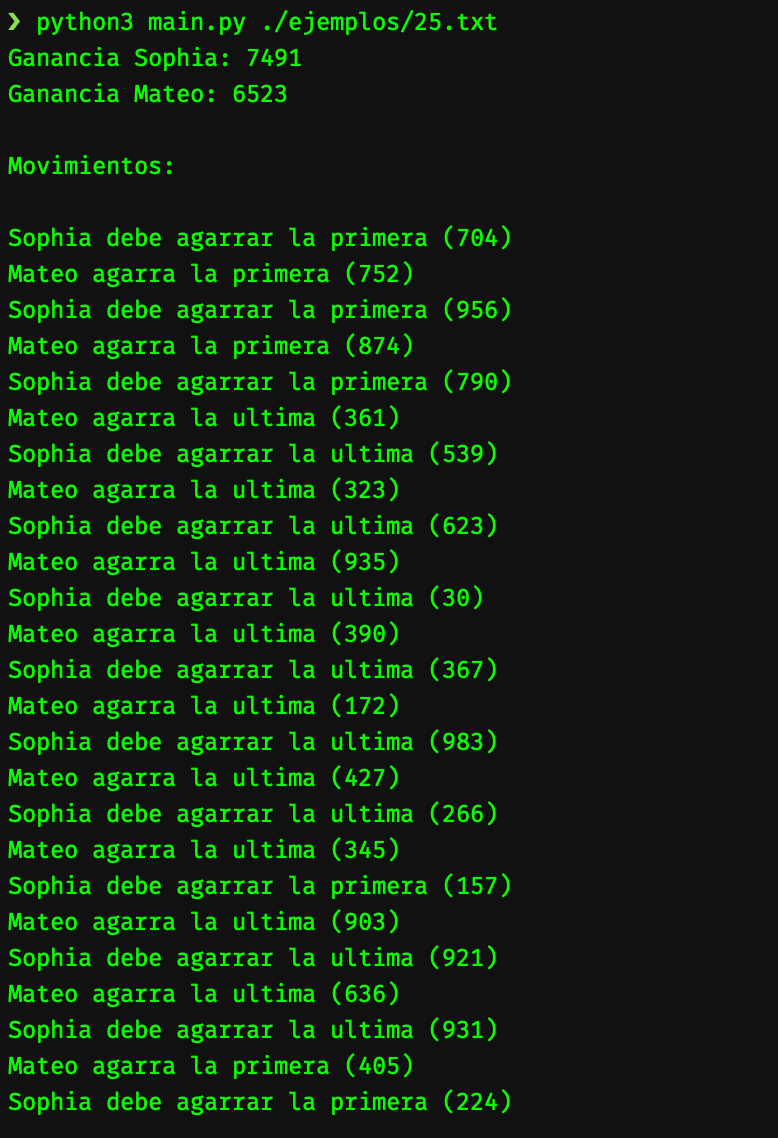
\includegraphics[scale = 0.6]{ {images/screen2.png} } 
\end{center}

Como podemos observar, los resultados obtenidos coinciden con los \textit{Resultados esperados} compartidos por la cátedra.